\documentclass[aspectratio=169]{../latex_main/tntbeamer}  % you can pass all options of the beamer class, e.g., 'handout' or 'aspectratio=43'
\usepackage{dsfont}
\usepackage{bm}
\usepackage[english]{babel}
\usepackage[T1]{fontenc}
%\usepackage[utf8]{inputenc}
\usepackage{graphicx}
\graphicspath{ {./figures/} }
\usepackage{algorithm}
\usepackage[ruled,vlined,algo2e,linesnumbered]{algorithm2e}
\usepackage{hyperref}
\usepackage{booktabs}
\usepackage{mathtools}

\usepackage{amsmath,amssymb}

\DeclareMathOperator*{\argmax}{arg\,max}
\DeclareMathOperator*{\argmin}{arg\,min}

\usepackage{amsbsy}
\newcommand{\vect}[1]{\bm{#1}}
%\newcommand{\vect}[1]{\boldsymbol{#1}}

\usepackage{pgfplots}
\pgfplotsset{compat=1.16}
\usepackage{tikz}
\usetikzlibrary{trees} 
\usetikzlibrary{shapes.geometric}
\usetikzlibrary{positioning,shapes,shadows,arrows,calc,mindmap}
\usetikzlibrary{positioning,fadings,through}
\usetikzlibrary{decorations.pathreplacing}
\usetikzlibrary{intersections}
\pgfdeclarelayer{background}
\pgfdeclarelayer{foreground}
\pgfsetlayers{background,main,foreground}
\tikzstyle{activity}=[rectangle, draw=black, rounded corners, text centered, text width=8em]
\tikzstyle{data}=[rectangle, draw=black, text centered, text width=8em]
\tikzstyle{myarrow}=[->, thick, draw=black]

% Define the layers to draw the diagram
\pgfdeclarelayer{background}
\pgfdeclarelayer{foreground}
\pgfsetlayers{background,main,foreground}

% Requires XeLaTeX or LuaLaTeX
%\usepackage{unicode-math}

\usepackage{fontspec}
%\setsansfont{Arial}
\setsansfont{RotisSansSerifStd}[ 
Path=../latex_main/fonts/,
Extension = .otf,
UprightFont = *-Regular,  % or *-Light
BoldFont = *-ExtraBold,  % or *-Bold
ItalicFont = *-Italic
]
\setmonofont{Cascadia Mono}[
Scale=0.8
]

% scale factor adapted; mathrm font added (Benjamin Spitschan @TNT, 2021-06-01)
%\setmathfont[Scale=1.05]{Libertinus Math}
%\setmathrm[Scale=1.05]{Libertinus Math}

% other available math fonts are (not exhaustive)
% Latin Modern Math
% XITS Math
% Libertinus Math
% Asana Math
% Fira Math
% TeX Gyre Pagella Math
% TeX Gyre Bonum Math
% TeX Gyre Schola Math
% TeX Gyre Termes Math

% Literature References
\newcommand{\lit}[2]{\href{#2}{\footnotesize\color{black!60}[#1]}}

%%% Beamer Customization
%----------------------------------------------------------------------
% (Don't) Show sections in frame header. Options: 'sections', 'sections light', empty
\setbeamertemplate{headline}{empty}

% Add header logo for normal frames
\setheaderimage{
	% 
\includegraphics[height=\logoheight]{figures/TNT_darkv4.pdf}
	
\includegraphics[height=\logoheight]{../latex_main/figures/luh_logo_rgb_0_80_155.pdf}
	% 
\includegraphics[height=\logoheight]{figures/logo_tntluh.pdf}
}

% Header logo for title page
\settitleheaderimage{
	% 
\includegraphics[height=\logoheight]{figures/TNT_darkv4.pdf}
	
\includegraphics[height=\logoheight]{../latex_main/figures/luh_logo_rgb_0_80_155.pdf}
	% 
\includegraphics[height=\logoheight]{figures/logo_tntluh.pdf}
}

% Title page: tntdefault 
\setbeamertemplate{title page}[tntdefault]  % or luhstyle
% Add optional title image here
%\addtitlepageimagedefault{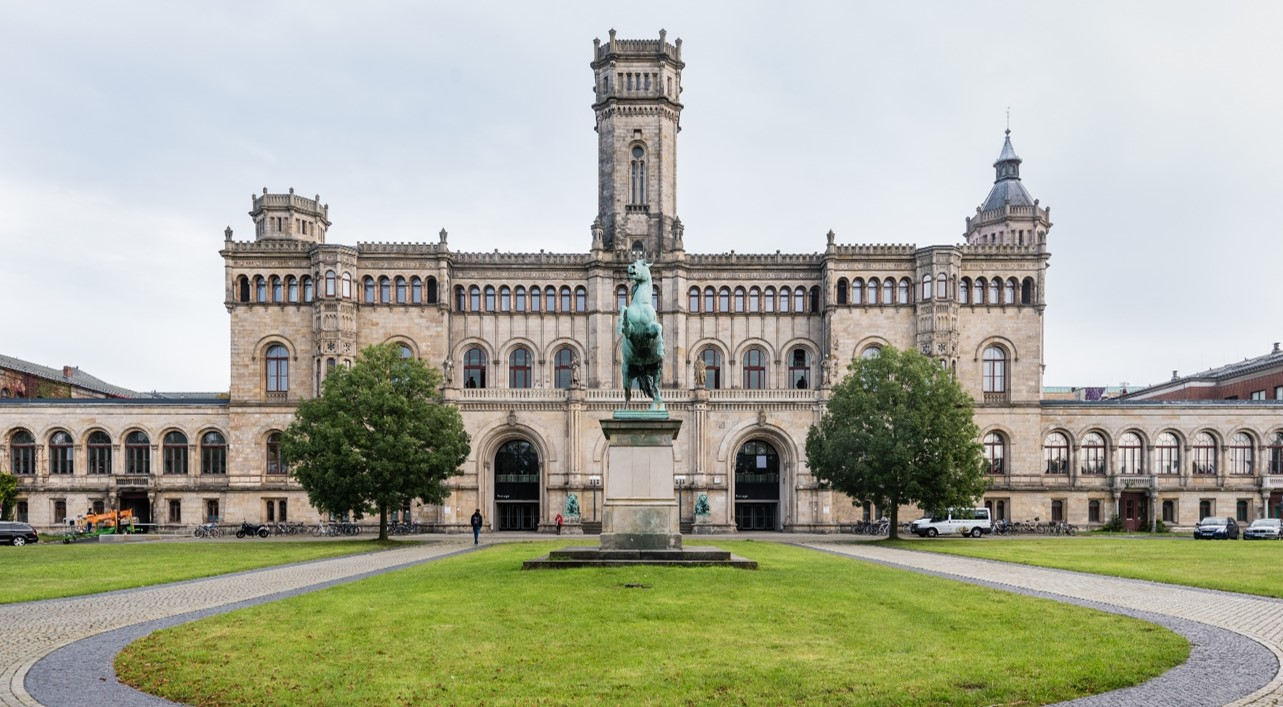
\includegraphics[width=0.65\textwidth]{figures/luh_default_presentation_title_image.jpg}}

% Title page: luhstyle
% \setbeamertemplate{title page}[luhstyle]
% % Add optional title image here
% \addtitlepageimage{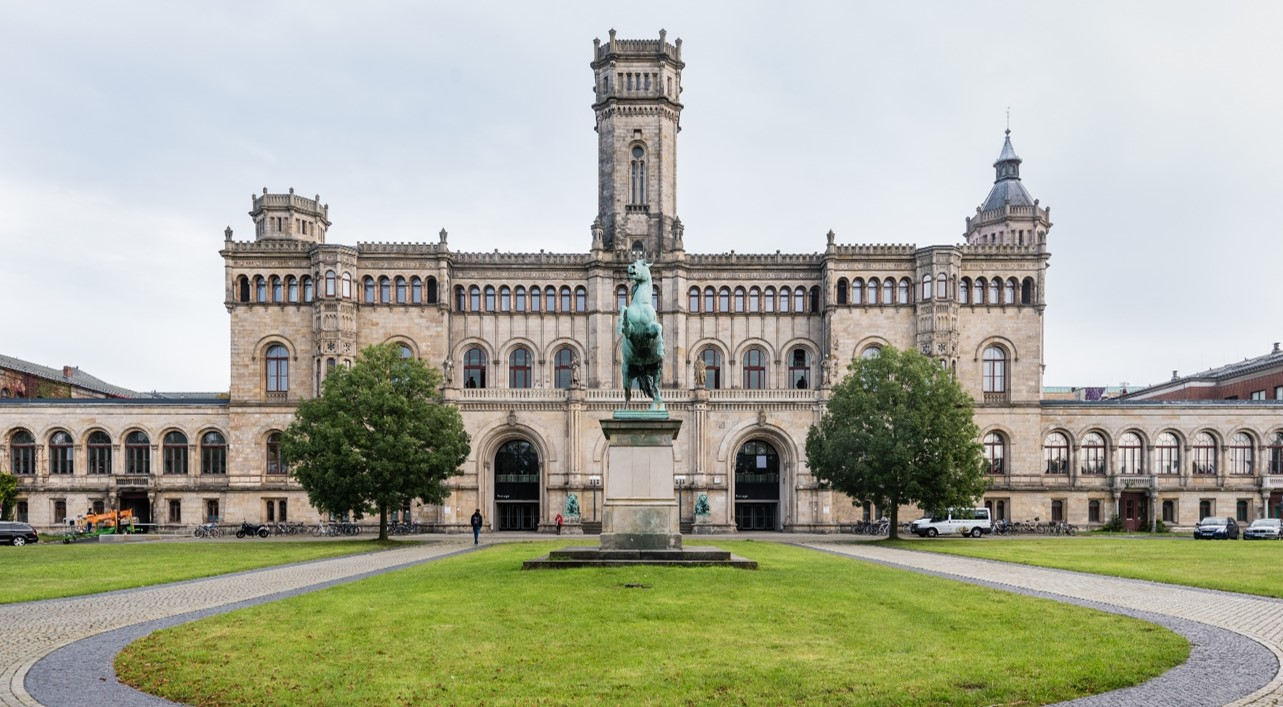
\includegraphics[width=0.75\textwidth]{figures/luh_default_presentation_title_image.jpg}}

\author[Abedjan \& Lindauer]{Ziawasch Abedjan \& Marius Lindauer\\[1em]
	
\includegraphics[height=\logoheight]{../latex_main/figures/luh_logo_rgb_0_80_155.pdf}\qquad
	
\includegraphics[height=\logoheight]{../latex_main/figures/DBIS_Kurzlogo.png}\qquad

\includegraphics[height=\logoheight]{../latex_main/figures/TNT_darkv4}\qquad

\includegraphics[height=\logoheight]{../latex_main/figures/L3S.jpg}	}
\date{Summer Term 2022; \hspace{0.5em} {
\includegraphics[height=1.5em]{../latex_main/figures/Cc-by-nc-sa_icon.svg.png}}; based on \href{https://ds100.org/fa21/}{[DS100]}
}


%%% Custom Packages
%----------------------------------------------------------------------
% Create dummy content
\usepackage{blindtext}

% Adds a frame with the current page layout. Just call \layout inside of a frame.
\usepackage{layout}


%%% Macros
%\renewcommand{\vec}[1]{\mathbf{#1}}
% \usepackage{bm}
%\let\vecb\bm

\title[Introduction]{DS: Logistic Regression, Part 1}
\subtitle{Logistic regression with squared loss}

\graphicspath{ {./figure/} }
%\institute{}


\begin{document}
	
	\maketitle
	\begin{frame}{Logistic regression with squared loss}
	    To find   $\hat{\theta}$   so that we can make predictions, we need to choose a loss function. 
        \begin{itemize}
            \item We can start with our old friend, squared loss.
            \item Doing so yields the following empirical risk:
        \end{itemize}
        \begin{equation*}
            R(\theta) = \frac{1}{n}\sum\limits_{i=1}^n(y_i-\sigma (\mathbb{X}_i^T\theta))^2
        \end{equation*}
        
        Sometimes, this works fine (and it is actually still used in some applications). Other times...\\
        \bigskip
        Here,    $\mathbb{X}_i$    is a single row of our design matrix.


	\end{frame}
	
	\begin{frame}{Pitfalls of squared loss with logistic regression}
	    \begin{columns}
	        \begin{column}{.4\textwidth}
	                The loss surface of MSE for a logistic regression model with a single slope plus an intercept often looks something like this.\\
	                \bigskip
	                If your initial guess for   $\hat{\theta}$  is way out in the flat yellow region, your numerical optimization routine can get stuck.
	                \begin{equation*}
	                    \theta^{(t+1)} = \theta^{(t)} - \alpha\nabla_\theta R(\theta,\mathbb{X},\mathbb{Y})
	                \end{equation*}
	                If the gradient is 0, your update rule will stop changing.
	        \end{column}
	        
	        
	        \begin{column}{.4\textwidth}
	                \begin{figure}
	                    \centering
	                    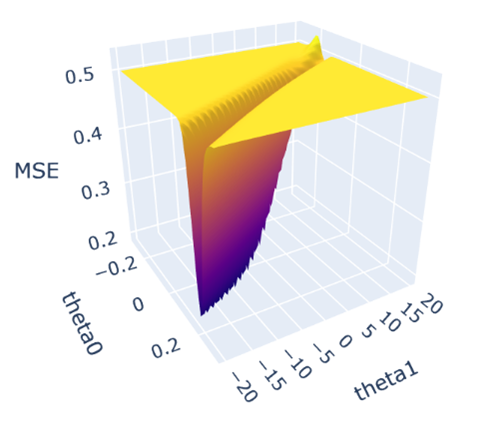
\includegraphics[scale=.5]{Bild12}
	                \end{figure}
	       \end{column}
	    \end{columns}
	\end{frame}
	
	
	\begin{frame}{Pitfalls of squared loss with logistic regression}
	    On the left, we have a toy dataset (i.e. we’ve plotted the original data, y vs. x). On the right, we have a plot of the mean squared error of this dataset when fitting a single-feature logistic regression model, for different values of (i.$\theta$ the loss surface).
	    \begin{figure}
	        \centering
	        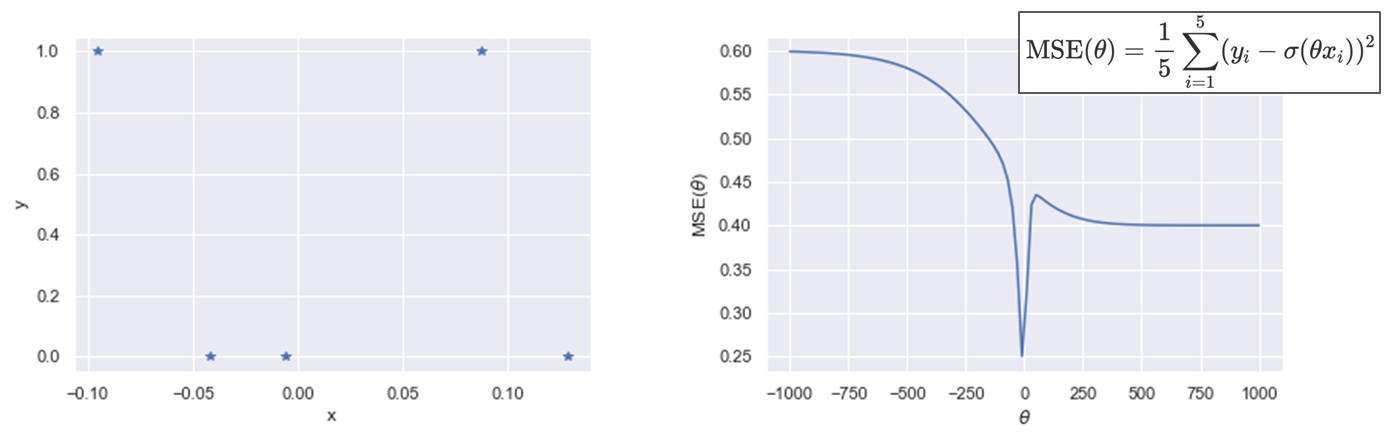
\includegraphics[scale=.4]{Bild13}
	    \end{figure}
	\end{frame}
	
	
	\begin{frame}{Pitfalls of squared loss with logistic regression}
	    On the left, we have a toy dataset (i.e. we’ve plotted the original data, y vs. x). On the right, we have a plot of the mean squared error of this dataset when fitting a single-feature logistic regression model, for different values of (i.$\theta$ the loss surface).
	    \begin{figure}
	        \centering
	        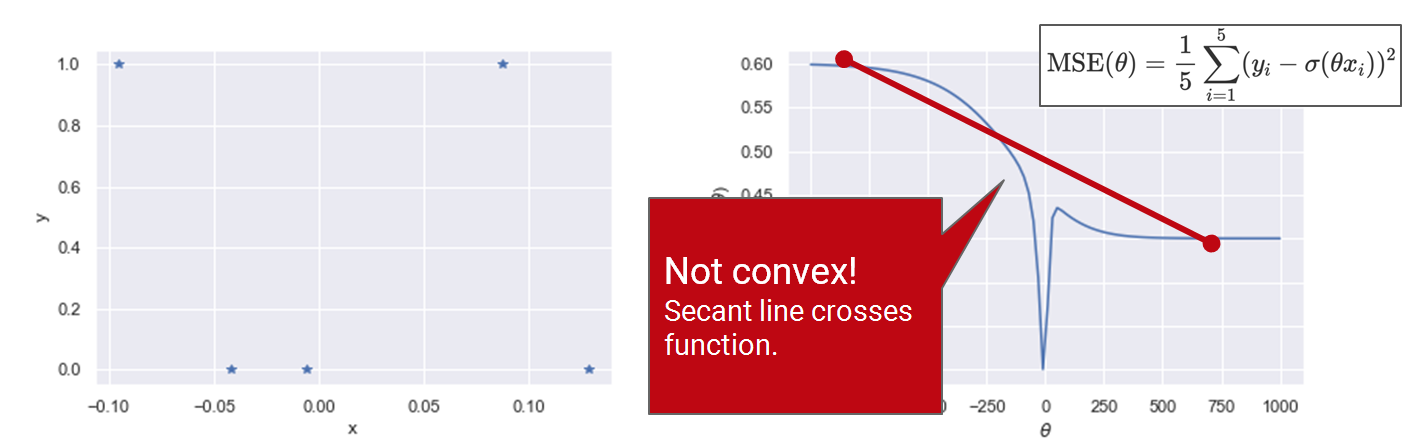
\includegraphics[scale=.4]{Bild14}
	    \end{figure}
	\end{frame}
	
	
	\begin{frame}{Pitfalls of squared loss with logistic regression}
	    \begin{columns}
	        \begin{column}{.5\textwidth}
	                For this particular loss surface, different initial guesses for thetahat yield different “optimal values”, as per scipy.optimize.minimize:
	                \begin{figure}
	                    \centering
	                    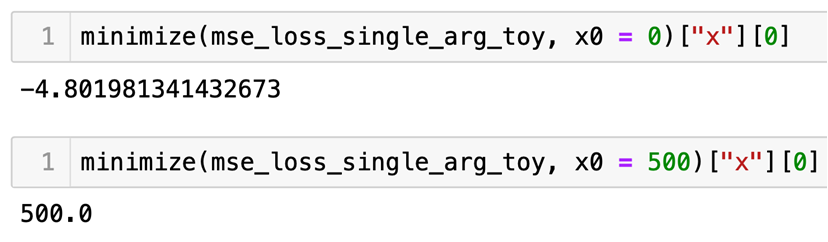
\includegraphics[scale=.65]{Bild15}
	                \end{figure}
	                This loss surface is not convex. We’d like it to be.
	        \end{column}
	        
	        \begin{column}{.5\textwidth}
	                \begin{figure}
	                    \centering
	                    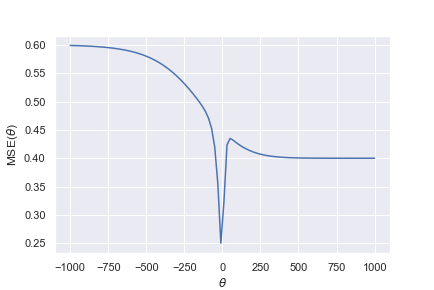
\includegraphics[scale=.65]{Bild16}
	                \end{figure}
	        \end{column}
	    \end{columns}
	\end{frame}
	
	
	\begin{frame}{Pitfalls of squared loss with logistic regression}
        Another issue: since  $y_i$     is either 0 or 1, and   $\hat{y_i}$    is between 0 and 1,          $(y_i - \hat{y_i})^2$            is also bounded between 0 and 1.
        \begin{itemize}
            \item Even if our probability is nowhere close, the loss isn’t that large in magnitude.
            \begin{itemize}
                \item If we say the probability is 10$^{-6}$, but it happens anyway, error should be large.
            \end{itemize}
            \item We want to penalize wrong answers significantly.
        \end{itemize}
	    \begin{columns}
	        \begin{column}{.5\textwidth}
	                \\ \bigskip
	               Suppose the observation we're trying to predict is actually in class 1. \\
	               \bigskip
	               
	                On the right, we have a plot of     $(1 - \hat{y})^2$            vs $\hat{y}$      . This is the squared loss for a single prediction
	        \end{column}
	        
	        \begin{column}{.5\textwidth}
	                \begin{figure}
	                    \centering
	                    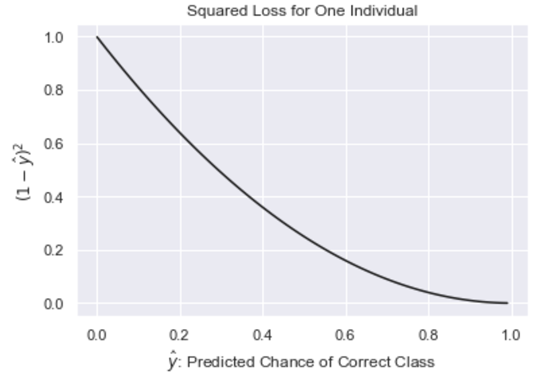
\includegraphics[scale=.55]{Bild17}
	                \end{figure}
	        \end{column}
	    \end{columns}
	\end{frame}
	
	\begin{frame}{Summary of issues with squared loss and logistic regression}
	    While it can work, squared loss is not the best choice of loss function for logistic regression.
	    \begin{itemize}
	        \item Average squared loss is not convex.
	        \begin{itemize}
	            \item Numerical methods will struggle to find a solution.
	        \end{itemize}
	        \begin{itemize}
	            \item Wrong predictions aren’t penalized significantly enough.
	        \end{itemize}
	        \item Squared loss (and hence, average squared loss) are bounded between 0 and 1.
	    \end{itemize}
	    
	    \bigskip
	    Fortunately, there’s a solution.
	\end{frame}
\end{document}